%======================================================================
\section{Data assimilation details}
\label{app:da}
%======================================================================

\subsection{Observation networks}
\label{app:da_networks}

Table~\ref{tab:da_networks} lists every configuration. The grid spacing
is that of the training data at every size, so a fixed stride is a fixed
physical spacing: two observations per site in 1D and four in 2D.
Observation errors are independent with standard deviation $0.1$ in
standardized units; $R=0.01\,I$.

\begin{table}[htbp]
\caption{Data assimilation configurations: grid, sites, latent dimension
$\dlat$, observation stride (grid points), spacing (length units) and
number of observations $m$.}
\label{tab:da_networks}
\begin{ruledtabular}
\begin{tabular}{llccccccccc}
system & size & grid & sites & $c$ & $\dlat$ & $K$ & offsets & stride & spacing & $m$ \\
\hline
\tabinput{tables/tabE_p2_networks}
\end{tabular}
\end{ruledtabular}
\end{table}

\subsection{Analysis schemes}
\label{app:da_filters}

Let $Z\in\R^{\Nens\times\dlat}$ be the forecast ensemble, $\bar z$ its mean,
$X=Z-\bar z$ the (optionally inflated) perturbations, $B=X^\top X/(\Nens-1)$,
$J$ the Jacobian of $h=\Hobs\circ\Dec$ at $\bar z$, and $\rho$ the
Gaspari--Cohn taper \citep{gaspari1999} of half-width $3$ sites, which
vanishes at site distances of 6 and more.

\para{Dense filter.} With perturbed observations
$y^{(e)}=y+\varepsilon^{(e)}$, $\varepsilon^{(e)}\sim\mathcal N(0,R)$,
\begin{equation}
\begin{aligned}
  z_a^{(e)} &= z^{(e)} + K\big(y^{(e)}-h(z^{(e)})\big),\\
  K &= (\rho\circ B)J^\top\big(J(\rho\circ B)J^\top+R\big)^{-1}.
\end{aligned}
\end{equation}
The innovation uses the nonlinear $h$; the gain uses $J$.

\para{Per-site filter.} For each site $s$, let $U_s$ be the observations
with $\rho(\dist(s,\mathrm{site}(i)))>0$, $N_s$ the sites that own them,
and $R_s=\mathrm{diag}(R_{ii}/\rho_i)_{i\in U_s}$. With $J_s$ the rows of $J$
in $U_s$ restricted to the columns of $N_s$ (exact by
Proposition~\ref{prop:blockdiag}), $B_{N_s}$ the sample covariance of the
sites in $N_s$ and $B_{s,N_s}$ that of site $s$ with them,
\begin{equation}
\begin{aligned}
  z_{a,s}^{(e)} &= z_s^{(e)} + K_s\big(y^{(e)}_{U_s}-h_{U_s}(z^{(e)})\big),\\
  K_s &= B_{s,N_s}J_s^\top\big(J_sB_{N_s}J_s^\top+R_s\big)^{-1}.
\end{aligned}
\end{equation}
The covariance $B_{N_s}$ is not tapered; localization acts only through
$R_s$ \citep{hunt2007}.

\para{Deterministic transform.} With the same $U_s$, $R_s$ and
$Y=X_{N_s}J_s^\top\in\R^{\Nens\times|U_s|}$,
\begin{equation}
\begin{aligned}
  \tilde P &= \big[(\Nens-1)I+YR_s^{-1}Y^\top\big]^{-1},\\
  \bar w &= \tilde P\,YR_s^{-1}\big(y-\overline{h(z)}\big)_{U_s},\\
  W &= \big[(\Nens-1)\tilde P\big]^{1/2},
\end{aligned}
\end{equation}
and site $s$'s analysis ensemble is $\bar z_s + (\bar w\mathbf 1^\top+W)^\top X_s$
\citep{hunt2007}. For a linear $h$ without localization it reproduces
the Kalman update computed with the ensemble covariance exactly (unit
test). At $44^2$ its skill is within $0.15$ of the perturbed-observation
version at every ensemble size (Table~\ref{tab:da_2d_ensemble}) and its
CPU time about $40\%$ lower.

\para{Particle flow filter.} The Gauss--Newton (``NAT'') variant of
\citet{huvanleeuwen2021} with the localized prior covariance $\rho\circ B$,
held fixed in pseudo-time, at most 100 pseudo-time steps.

\para{Sampling error correction.} The correction table of
\citet{anderson2012} is built by Monte Carlo for each ensemble size
(2000 trials per true correlation on a grid of 41 values in
$[-0.98,0.98]$, 100 bins). In \emph{matrix form} each sample correlation in
$B$ is replaced by its corrected value; the result need not be positive
semidefinite. The \emph{projected form} raises its eigenvalues to at
least $10^{-10}$ times the largest. The \emph{serial form} assimilates the
observations one at a time on the augmented state $[Z,h(Z)]$ and applies
the correction to each scalar regression coefficient,
$\beta_k=\mathrm{SEC}\big(\mathrm{corr}(x_k,\hat y_j)\big)\,\sigma_{x_k}\sigma_{\hat y_j}/(\sigma^2_{\hat y_j}+R_{jj})$.

\subsection{Cost of the observation Jacobian}
\label{app:da_jacobian}

Figure~\ref{fig:jacobian_timing} times the latent observation Jacobian at
every deployment size, with the observation network of the runs. The
coloured construction, $c=6$ forward-mode passes through the decoder,
gives the same matrix as dense reverse-mode differentiation to the last
digit (largest difference $0$ up to $132^2$), and its time grows slightly
more slowly than the latent dimension: $1.3$~ms at $44^2$ and $49$~ms at $440^2$.
Reverse mode needs one pass per observation and grows almost with the
square of the dimension, $52$ times slower at $132^2$; we did not run it
beyond that size.

\begin{figure}[htbp]
\centering
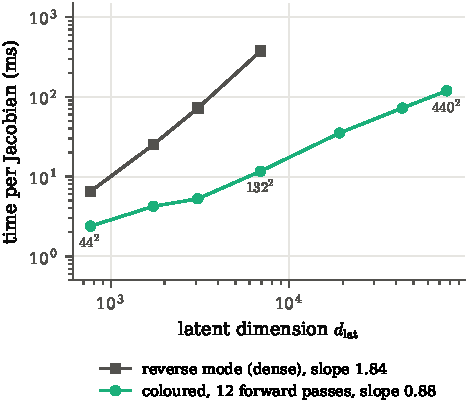
\includegraphics{figures/fig12_jacobian_timing.pdf}
\caption{Wall time per observation Jacobian against latent dimension,
2D KS, observation spacing $2.75$, four CPU threads, median of three: dense
reverse mode (one pass per observation) and the coloured construction
used by the per-site filter (six forward passes). The two agree exactly
where both were computed. Slopes are least-squares power-law fits.}
\label{fig:jacobian_timing}
\end{figure}

\subsection{Inflation, run-to-run spread and transients}
\label{app:da_tuning}

Multiplicative inflation of the forecast perturbations has little
effect (Table~\ref{tab:da_inflation}): the unlocalized filter is
unchanged to $1\%$, the per-site filter loses $4\%$ of its skill at
inflation $1.2$ and the dense localized filter $9\%$, and calibration moves
by at most $0.02$. With four observations per site and $R=0.01\,I$ the
analysis is dominated by the observations. All other runs use no
inflation.

A second seed, which changes the initial ensemble, the observation
noise and the model noise, changes the steady-state skill of the
per-site filter by $0.02$--$0.15$ at every size from $44^2$ to $330^2$ and that of the
unlocalized filter by $0.03$--$0.23$; differences below about $0.2$ in skill
are within run-to-run variation. The initial ensemble starts close to the
truth, so the analysis error first rises; it reaches its steady level
within $10$--$20$ cycles, after which its 10-cycle means vary by about
$\pm10\%$ at $44^2$ and $\pm3\%$ at $88^2$ and larger, the smaller domains averaging over
fewer independent regions. The per-cycle values of every run are stored
with its summary.

\begin{table}[htbp]
\caption{Steady-state skill (calibration) against multiplicative
inflation, 2D KS at $44^2$, 64 members.}
\label{tab:da_inflation}
\begin{ruledtabular}
\begin{tabular}{lcccc}
filter & 1.0 & 1.05 & 1.1 & 1.2 \\
\hline
\tabinput{tables/tabE_inflation}
\end{tabular}
\end{ruledtabular}
\end{table}
